
% This LaTeX was auto-generated from MATLAB code.
% To make changes, update the MATLAB code and republish this document.

\documentclass{article}
\usepackage{graphicx}
\usepackage{color}

\sloppy
\definecolor{lightgray}{gray}{0.5}
\setlength{\parindent}{0pt}

\begin{document}

    
\begin{verbatim}
AC = ACDBday(4, 21, 2019);
nErr = AC(:,1) - AC(:,2);
f = @(t) 0.4*t  + 35;
t = 1:length(AC);
q = 0;
ncum = 0;
tcum = 0;

for i = t
    if heaviside(nErr(i))
        ncum = ncum + nErr(i);
        tcum = ncum;
    else
        q = q + 1;
        tcum = abs(nErr(i));
    end
    if tcum + ncum > f(t(i))
        q = q-1;
        if q < 0
            q = 0;
        end
        tcum = 0;
        ncum = 0;
        pf(i) = 1;

    else
        pf(i) = 0;
    end
    Q(i) = q;
    N(i) = ncum;
    T(i) = tcum;
    NT(i) = tcum + ncum;
end
plot(t, f(t), t, NT)
\end{verbatim}

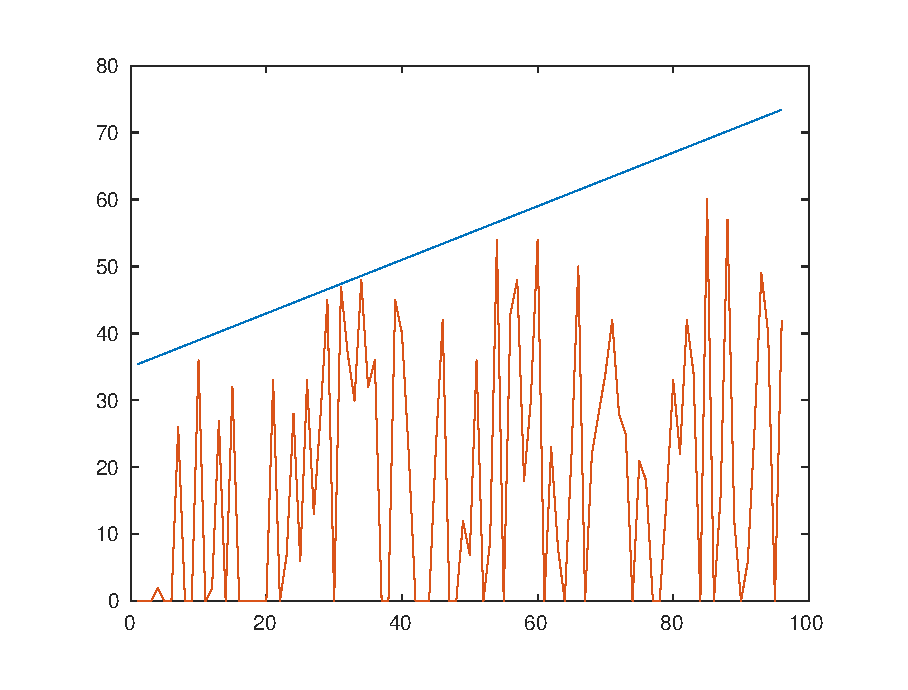
\includegraphics [width=4in]{linPF_01.eps}



\end{document}
    
